% ====================================================================
%+
% SECTION:
%    tde.tex
%
% CHAPTER:
%    transients.tex
%
% ELEVATOR PITCH:
%    Tidal disruption events (TDEs) are the disruptions of stars by supermassive black holes.
%    They can produce flares in the optical and UV (sometimes accompanied by X-ray and radio emission as well).
%    These flares can be used to reveal the properties of otherwise quiescent SMBHs and to study accretion physics.
%    TDEs are rare, LSST will allow the first statistical sample of such events.
%
% AUTHORS:
%    Iair Arcavi (@arcavi)
%
% ====================================================================

% \section{Tidal Disruption Events}
\subsection{Tidal Disruption Events}
\def\secname{\chpname:tdes}\label{sec:\secname}

\credit{arcavi}

A star passing close to a supermassive black hole (SMBH;
$M\gtrsim10^{6}M_{\odot}$) will be torn apart by tidal forces. For
certain ($\lesssim10^{8}M_{\odot}$) black hole masses, the disruption
will occur outside the event horizon and will be accompanied by an
observable flare \citep{Hills1975, Rees1988}. Such flares can be used to
study inactive SMBHs, which are otherwise inaccessible beyond the nearby
($\lesssim100$ Mpc) universe.

We are now building our understanding of how observational properties of
TDEs are affected by the SMBH. Theory claims to provide such a
connection \citep[e.g.][]{Lodato2009, Guillochon2014}, but uncertainties
in the physics of the disruption, subsequent accretion and emission
mechanisms are currently topics of debate \citep[e.g.][]{Strubbe2015,
Guillochon2014, Roth2015}, and new models are vigorously being developed
\citep[e.g.][]{Piran2015, Hayasaki2015, Svirski2015, Bonnerot2015}.

TDEs are rare ($\sim10^{-5}-10^{-4}$ events per galaxy per year;
\citealp{Wang2004, Stone2015}), and until recently, TDE candidates were
discovered mostly in archival data \citep[e.g.][]{Donley2002,
Gezari2006, Esquej2007}. Now, however, wide-field transient surveys have
started discovering TDEs in real time.

Generally, two types of TDE candidates have been identified:
\begin{enumerate}
	\item \textit{High energy TDEs}. The prototype is Swift J1644
\citep{Bloom2011, Burrows2011, Levan2011, Zauderer2011}, with two other
events known \citep{Cenko2012, Brown2015}. These events display emission
in $\gamma$-rays and X-rays as well as in the radio, but are not
detected in the optical.
\item \textit{Optical-UV TDEs}.  The prototype is PS1-10jh
(Figure \ref{fig:tde}; \citealp{Gezari2012}).
		About $8$ other events are known
\citep{Chornock2014, Arcavi2014, Holoien2014, Holoien2015, Holoien2016}.
Some events were detected also in the X-rays and radio (in addition to
the optical and UV), but the X-ray and radio signatures are different
than those of the high energy TDE candidates.
\end{enumerate}

\begin{figure}[hbt]
\centerline{
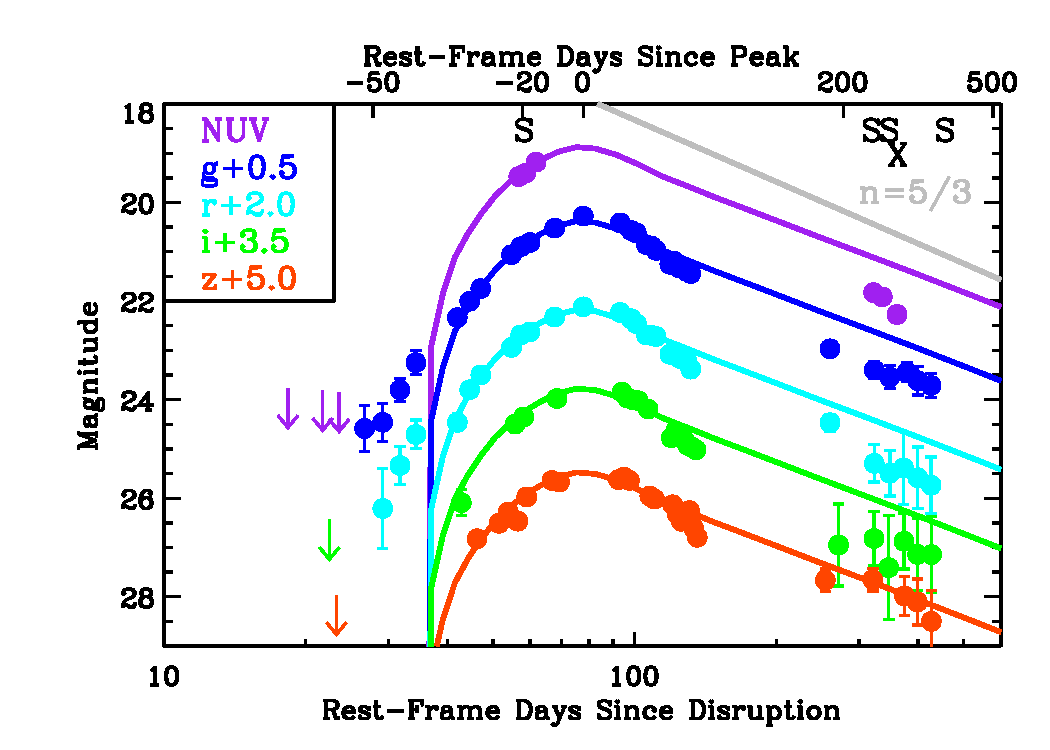
\includegraphics[width=0.6\textwidth]{figs/transients/tdeGezari.pdf}
}
\caption{
Optical and near-UV lightcurve of the TDE PS1-10jh \citep{Gezari2012}.
}
\label{fig:tde}
\end{figure}

It is still not clear whether both of these classes of transients are TDEs,
and if so, why they are so different form each other. One option raised is
that some TDEs may launch jets, which when directed towards us, appear as
the high energy events, but otherwise appear as the optical-UV events.
It is still not clear if this is indeed the case \citep[e.g.][]{VanVelzen2013}.

Here we focus on the second type of TDE candidates, which is the
relevant class for LSST, since they can be discovered in the optical.
However, multi-wavelength coordinated observations of
optically-discovered events are required in order to better understand
the connection between the two types of candidates.

The first well-sampled TDE of the optical+UV class was PS1-10jh (discovered by Pan-STARRS;
\citealt{Gezari2012}). \citet{Arcavi2014} later presented three new TDE candidates
from PTF and one discovered by ASAS-SN, all with similar properties
as PS1-10jh. These events exhibit blue colors, broad light curves,
peak absolute magnitudes of $\sim-20$ and a $\sim t^{-5/3}$ decay
at late times. This decay law has been suggested as a unique signature
of accretion-powered TDE light curves \citep{Rees1988, Evans1989, Phinney1989}.
Early-time deviations from the $t^{-5/3}$ rate
can be used to constrain the density profile of the disrupted star
\citep{Lodato2009, Gezari2012}. Late-time deviations would
test the accretion power-source hypothesis altogether.

The spectral signatures of these TDEs are still a puzzle. PS1-10jh displayed
only He II emission lines, lacking any signs of H. Some of the \citet{Arcavi2014}
sample, however, do display H emission.
In fact, a continuum of H / He emission ratios for this class of transients
is being revealed, and is now a focus of theoretical modelling \citep{Strubbe2015, Roth2015}.

The second recent discovery relating to this new sample concerns their
host galaxies \citep{Arcavi2014, French2016}, most of which are
post-starburst galaxies. These galaxies show little or no signs of on-going star formation, but their significant A stellar populations indicate that star formation ceased abruptly a few hundred Myr to a Gyr ago \citep{Dressler1983}. Galaxies with these characteristics often show signs of recent galaxy-galaxy mergers \citep{Zabludoff1996}, which produced the starburst and evolved the bulge. Optical-UV TDEs are intrinsically over abundant in post-starburst galaxies by a factor of $\sim30-200$ (depending on the characteristics of the galaxy; \citealt{French2016}). The reason for the strong preference of TDEs for post-starburst galaxies has still not been determined.

LSST's contribution to TDE studies will be substantial.
\citet{VanVelzen2011} estimate that LSST could discover approximately
4000 TDEs per year. The main drivers for studying TDEs with LSST are:
\begin{itemize}
\item Measuring black hole masses: This involves fitting models to TDE
light curves. It is also relevant to correlate these measurements with
host galaxy properties (mass, bulge/disk decomposition).
\item Constraining galactic dynamics by measuring the TDE rates as
functions of black hole mass and galaxy types.
\item Characterizing TDE emission signatures.
\end{itemize}

A metric is required for measuring how well TDEs can be identified and
distinguished from supernovae and active galactic nuclei. In general, we
expect TDEs to:
\begin{itemize}
\item Be located in the center of their host.
\item Display approximately constant blue (few $10^4$K) colors.
\item Evolve slowly (weeks-months).
\item Not show past AGN-like variability.
\item Preferentially peak around mag -20.
\item Preferentially be hosted in a post-starburst galaxy.
\end{itemize}
These criteria are based on our current knowledge of optical TDEs, which
is still in its early stages. The field is rapidly evolving, and it is
possible that new observations will change the current picture of TDE
emission. This metric is probably best combined with those discussed in
 \autoref{sec:\chpname:SNtransients} for identifying supernovae, though the
luminosity function of TDEs (or what constitutes a ``typical'' TDE light
curve) is not yet known.

A second metric is required to asses the accuracy with which the black
hole mass can be constrained from the TDE light curves. This metric can
be based on existing theoretical models to fit simulated TDE light
curves (such as TDEFit; \citealt{Guillochon2014}).

% ====================================================================
%
 \subsection{Conclusions}

 Here we answer the ten questions posed in
 \autoref{sec:intro:evaluation:caseConclusions}:

 \begin{description}

 \item[Q1:] {\it Does the science case place any constraints on the
 tradeoff between the sky coverage and coadded depth? For example, should
 the sky coverage be maximized (to $\sim$30,000 deg$^2$, as e.g., in
 Pan-STARRS) or the number of detected galaxies (the current baseline
 of 18,000 deg$^2$)?}

 \item[A1:] The number of events discovered will be approximately proportional to the sky area surveyed, multiplied by the
 average length of coverage, so added sky area is beneficial, as long as the observing season per field is not shortened.

 \item[Q2:] {\it Does the science case place any constraints on the
 tradeoff between uniformity of sampling and frequency of  sampling? For
 example, a rolling cadence can provide enhanced sample rates over a part
 of the survey or the entire survey for a designated time at the cost of
 reduced sample rate the rest of the time (while maintaining the nominal
 total visit counts).}

 \item[A2:] Uniform sampling is optimum.

 \item[Q3:] {\it Does the science case place any constraints on the
 tradeoff between the single-visit depth and the number of visits
 (especially in the $u$-band where longer exposures would minimize the
 impact of the readout noise)?}

 \item[A3:] No, as long as all filters are well represented.

 \item[Q4:] {\it Does the science case place any constraints on the
 Galactic plane coverage (spatial coverage, temporal sampling, visits per
 band)?}

 \item[A4:] This science will be accomplished away from the galactic plane.

 \item[Q5:] {\it Does the science case place any constraints on the
 fraction of observing time allocated to each band?}

 \item[A5:] Increased $u$-filter cadence valuable for TDE.

 \item[Q6:] {\it Does the science case place any constraints on the
 cadence for deep drilling fields?}

 \item[A6:] Only cadences that sample timescales of weeks and greater will be useful.

 \item[Q7:] {\it Assuming two visits per night, would the science case
 benefit if they are obtained in the same band or not?}

 \item[A7:] Different bands would be strongly preferred.

 \item[Q8:] {\it Will the case science benefit from a special cadence
 prescription during commissioning or early in the survey, such as:
 acquiring a full 10-year count of visits for a small area (either in all
 the bands or in a  selected set); a greatly enhanced cadence for a small
 area?}

 \item[A8:] A sparse cadence applied to a large sky area would be scientifically productive, but this is not a strong constraint.

 \item[Q9:] {\it Does the science case place any constraints on the
 sampling of observing conditions (e.g., seeing, dark sky, airmass),
 possibly as a function of band, etc.?}

 \item[A9:] No.

 \item[Q10:] {\it Does the case have science drivers that would require
 real-time exposure time optimization to obtain nearly constant
 single-visit limiting depth?}

 \item[A10:] No.

 \end{description}

 \navigationbar
